Once expected losses are computed, they must be translated into a shift in probability of default ($\Delta PD_C$). We use the interest coverage ratio (ICR) approach based on Damodaran's methodology~\cite{damodaran2012investment}, which maps ICR ranges to credit ratings and default spreads. This approach is deliberately chosen for its simplicity and transparency; the framework is modular, and more sophisticated credit models --- including the Merton structural model~\cite{merton1974pricing} or machine learning approaches --- can substitute for this module. The ICR-based translation does not capture firm-specific financial dynamics beyond the EBIT-to-interest ratio (e.g., insurance recovery schedules, covenant structures, or adaptive strategies such as hedging and rapid asset disposal); extending the credit module to include these factors is a natural direction for future work.

The ICR is defined as $\ICR = \EBIT / \IE$. Damodaran~\cite{damodaran2012investment} provides a discrete mapping from $\ICR$ ranges to credit ratings and default spreads (15 rating bands from D to AAA). We use a continuous approximation of this mapping (Fig.~\ref{fig:damodaran smooth}) to avoid discontinuous PD responses at rating boundaries.

\begin{figure}
    \centering
    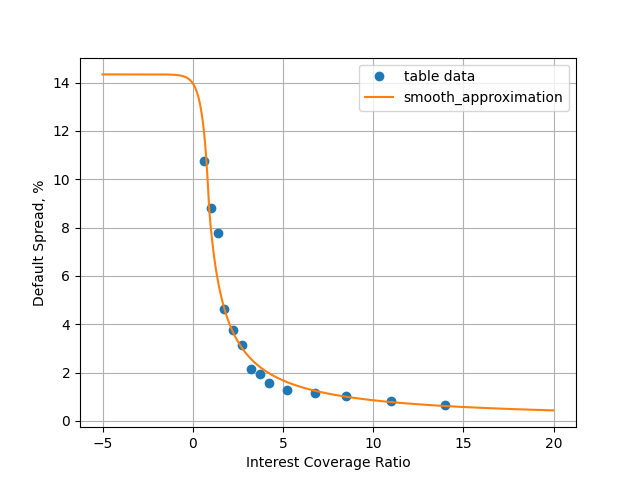
\includegraphics[width=.7\textwidth]{Content/Images/icr_pd.png}
    \caption{Continuous approximation of the ICR-to-default-spread mapping~\cite{damodaran2012investment}.}
    \label{fig:damodaran smooth}
\end{figure}

The probability of default is obtained by dividing the default spread by $(1 - \RR)$, where $\RR$ is the recovery rate (typically 0.4). When a climate event occurs, EBIT is reduced by the expected loss:

\begin{equation*}
    \ICR_C = \frac{\EBIT - \ECL}{\IE}
    %\label{eq: icr}
\end{equation*}

The climate-induced PD shift is:
\begin{equation*}
    \Delta \PD_C = P[\FS_C] - P[\FS]
    %\label{eq: pd shift general}
\end{equation*}
where $P[\cdot]$ denotes the PD implied by the continuous ICR-to-spread mapping. This formulation captures the non-linear sensitivity of credit risk to climate losses: companies with ICR in the 1--4 range (where the spread function has the steepest slope) experience disproportionately large PD shifts relative to the magnitude of the loss.
